\chapter{BACKGROUND OF SPEARMAN'S RHO AND KENDALL'S TAU}\label{chap:background}
%%%%%%%%%%%%%%%%%%%%%%%%%%%%%%%%%%%%%%%%%%%%%%%%%%%%%%%%%%%%%%%%%%%%%%%%%%%%%%%%%%%%%
%%%%%%%%%%%%%%%%%%%%%%%%%%%%%%%%%%%%%%%%%%%%%%%%%%%%%%%%%%%%%%%%%%%%%%%%%%%%%%%%%%%%%
%%%%%%%%%%%%%%%%%%%%%%%%%%%%%%%%%%%%%%%%%%%%%%%%%%%%%%%%%%%%%%%%%%%%%%%%%%%%%%%%%%%%%
%%%%%%%%%%%%%%%%%%%%%%%%%%%%%%%%%%%%%%%%%%%%%%%%%%%%%%%%%%%%%%%%%%%%%%%%%%%%%%%%%%%%%
%%%%%%%%%%%%%%%%%%%%%%%%%%%%%%%%%%%%%%%%%%%%%%%%%%%%%%%%%%%%%%%%%%%%%%%%%%%%%%%%%%%%%
\section{The History of Spearman's Rho}\label{sec:the_history_of_spearmans_rho}
\hspace{24pt} In statistics, it is a common to study the correlation between variables. It is important to understand the relationship between variables to check for dependence or lack of dependence. A common statistic used in linear regression, Pearson's correlation coefficient ($\rho$) can quantify the linear dependence between two random variables. A variant of Pearson's correlation coefficient is Spearman's Rho ($\rho_S$), which can be defined as the same quantity using the rank of the variables. The rank of a number is the corresponding index of an observation in the ordered data set. For example, the numbers $\{5,7,8,2,4\}$ have corresponding ranks $\{3,4,5,1,2\}$. We will begin by defining the sample version of Spearman's Rho, and consider the population version shortly after.
\begin{definition}\label{def:pearson}
    Let $\left(x_1,y_1\right),\left(x_2,y_2\right),\ldots,\left(x_n,y_n\right)$ be real-valued observations. Pearson's correlation coefficient can be defined as $$\widehat{\rho}\left(x,y\right)=\frac{\sum_{i=1}^n\left(x_i-\bar{x}\right)\left(y_i-\bar{y}\right)}{\sqrt{\sum_{i=1}^n\left(x_i-\bar{x}\right)^2}\sqrt{\sum_{i=1}^n\left(y_i-\bar{y}\right)^2}}=\frac{\widehat{\text{Cov}}\left(x,y\right)}{s_{x}s_{y}}.$$
\end{definition}
\begin{definition}\label{def:spearman_sample}
    Let $\left(x_1,y_1\right),\left(x_2,y_2\right),\ldots,\left(x_n,y_n\right)$ be real-valued observations and let $r_x$ and $r_y$ be the ranks of each respective variable. Spearman's Rho of a sample can be defined as $$\widehat{\rho}_S\left(r_x,r_y\right)=\frac{\sum_{i=1}^n\left(r_{x_i}-\bar{r_x}\right)\left(r_{yi}-\bar{r_y}\right)}{\sqrt{\sum_{i=1}^n\left(r_{xi}-\bar{r_x}\right)^2}\sqrt{\sum_{i=1}^n\left(r_{yi}-\bar{r_y}\right)^2}}=\frac{\widehat{\text{Cov}}\left(r_x,r_y\right)}{s_{r_x}s_{r_y}}.$$
\end{definition}
This idea of rank correlation was first introduced into the psychology community by Charles Spearman in 1904. The motivation behind this measurement was to erase the quantity in observations and analyze how data increased/decreased. In the original paper, Spearman commented ``it can often be altogether escaped in the case of quantities not admitting absolute measurement, by substituting instead \textit{comparison}"\cite{spearman1904}. As a consequence, Rho not only measures linear correlation, but any type of positive or negative monotone behavior (exponential, quadratic, linear, etc.). By using the ranks of the data, the quantity is erased from the calculation.

For random variables, the population version of Spearman's Rho will be needed. The population definition was introduced by William Kruskal in 1958 \cite{kruskal1958}. The following definition uses the concept of concordance and discordance, which are essential throughout this paper.
\begin{definition}\label{def:concordant_discordant}
    A concordant pair occurs when there are two points, $(x_1,y_1)$ and $(x_2,y_2)$, that have the same sign when subtracted. In other words, $\sign(x_2-x_1)=\sign(y_2-y_1)$. Discordant pairs occur when the opposite is true, or when they have opposite signs. In other words, $\sign(x_2-x_1)=-\sign(y_2-y_1)$.
\end{definition}
Graphically, a concordant pair will form an increasing, positively sloped line between the two points. Similarly, a discordant pair will form a decreasing, negatively sloped line between the two points.
\begin{figure}[h]
    \centering
    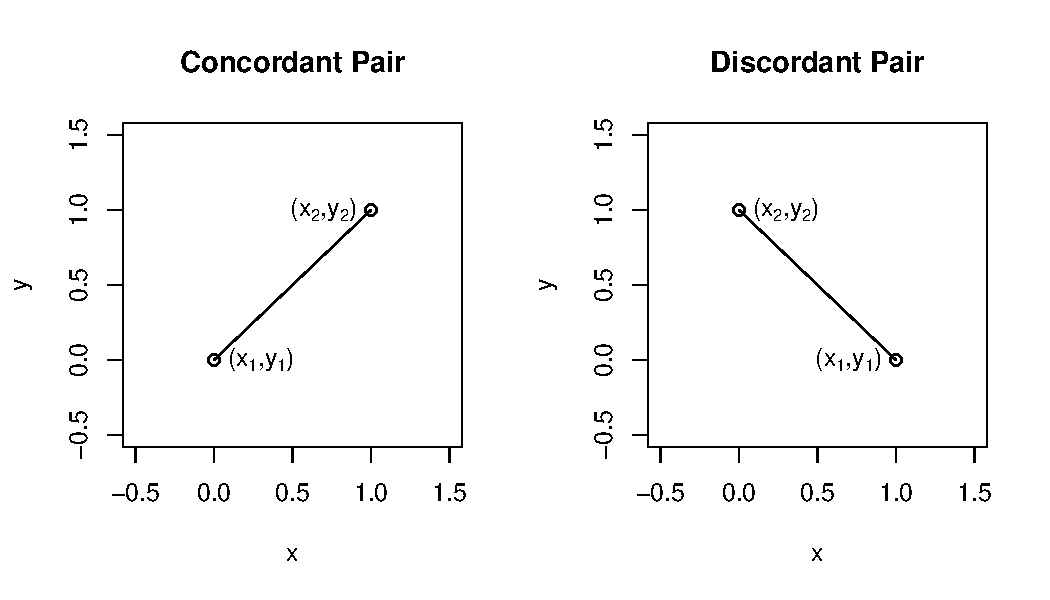
\includegraphics[scale=0.85]{images/pairs.pdf}
    %\caption{Two graphs showing examples of concordant and discordant pairs. Notice the plot to the right is increasing and the plot to the left is decreasing.}
    \caption{Two graphs showing examples of concordant and discordant pairs.}
    \label{fig:pairs}
\end{figure}
\begin{definition}\label{def:spearman_population}
    Consider a bivariate distribution with random pair $(X,Y)$. Let $(X_1,Y_1)$, $(X_2,Y_2)$, and $(X_3,Y_3)$ be independent and identically distributed pairs. Spearman's Rho of a population can be defined as $$\rho_S=3\left(P\left(\left(X_1-X_2\right)\left(Y_1-Y_3\right)>0\right)-P\left(\left(X_1-X_2\right)\left(Y_1-Y_3\right)<0\right)\right).$$
\end{definition}
It is important to notice the dependence between $X_1$  and $Y_1$ and the independence between $X_2$ and $Y_3$. The reason for this will become more clear in Section \ref{sec:modern_expressions}. Also note that the quantity in the parentheses is multiplied by 3. This is because the quantity inside ranges from $-\frac{1}{3}$ to $\frac{1}{3}$ (for detail see \cite{kruskal1958} p. 824). The first term in the parentheses is the probability of concordance and the second term is probability of discordance. Also notice that the second term is the compliment of the first. There are several ways to write Spearman's Rho by taking advantage of this result. We will see in Section \ref{sec:modern_expressions} that Spearman's Rho can be written in terms of probabilities, copulas, and CDFs. Although not obvious, we will later see how the sample definition and the population definition relate to each other.
%%%%%%%%%%%%%%%%%%%%%%%%%%%%%%%%%%%%%%%%%%%%%%%%%%%%%%%%%%%%%%%%%%%%%%%%%%%%%%%%%%%%%
%%%%%%%%%%%%%%%%%%%%%%%%%%%%%%%%%%%%%%%%%%%%%%%%%%%%%%%%%%%%%%%%%%%%%%%%%%%%%%%%%%%%%
%%%%%%%%%%%%%%%%%%%%%%%%%%%%%%%%%%%%%%%%%%%%%%%%%%%%%%%%%%%%%%%%%%%%%%%%%%%%%%%%%%%%%
%%%%%%%%%%%%%%%%%%%%%%%%%%%%%%%%%%%%%%%%%%%%%%%%%%%%%%%%%%%%%%%%%%%%%%%%%%%%%%%%%%%%%
%%%%%%%%%%%%%%%%%%%%%%%%%%%%%%%%%%%%%%%%%%%%%%%%%%%%%%%%%%%%%%%%%%%%%%%%%%%%%%%%%%%%%
\section{The History of Kendall's Tau}\label{sec:the_history_of_kendalls_tau}
\hspace{24pt} In 1938, the statistics community was introduced to Kendall's Tau ($\tau$), another measure of rank correlation \cite{kendall1938}. There are several parallels between Rho and Tau. They both have the ability to measure monotone behavior between two variables and also both require ranks to calculate. If both Rho and Tau are calculated on a set of data, often the quantities are relatively close, and usually the same sign. The idea of concordant and discordant pairs are used in the calculation of Tau.
\begin{definition}\label{def:kendalls_sample}
    Given a sample of raw data, $\left(x_1,y_1\right),\left(x_2,y_2\right),\ldots,\left(x_n,y_n\right)$, calculate the number of concordant pairs $c$ and number of discordant pairs $d$. Kendall's Tau of a sample can be defined as $$\widehat{\tau}=\frac{c-d}{c+d}=\frac{c-d}{{n \choose 2}}$$ where $n$ is the sample size.
\end{definition}
There is an alternate definition for both Rho and Tau that accounts for tied pairs, which is when the sign equals zero. Throughout the paper, continuous data will be studied. Therefore, the probability of a tie happening is zero. The alternative definitions of Tau can be useful for discrete data.

For the population definition we have to find the difference between the probability of concordance and the probability of discordance. Just like Rho, there will be several results that take advantage of the symmetry of the following definition.
\begin{definition}\label{def:kendalls_population}
    Consider a bivariate distribution with random pair $(X, Y)$. Let $(X_1,Y_1)$ and $(X_2,Y_2)$ be independent and identically distributed pairs. Kendall's Tau of a population can be defined as $$\tau=P\left(\left(X_1-X_2\right)\left(Y_1-Y_2\right)>0\right)-P\left(\left(X_1-X_2\right)\left(Y_1-Y_2\right)<0\right).$$
\end{definition}
This result looks intuitively symmetric and, much like Rho, we will define this quantity in Section \ref{sec:modern_expressions} in terms of probabilities, copulas, and CDFs. It is also important to notice the dependence between $X_1$ and $Y_1$, and the dependence between $X_2$ and $Y_2$.

Let's briefly relate this definition to the sample definition. Applying the Law of Large Numbers, think of the sample size approaching infinity. $$\lim_{n\to\infty}\frac{c-d}{{n \choose 2}}=\lim_{n\to\infty}\frac{c}{{n \choose 2}}-\lim_{n\to\infty}\frac{d}{{n \choose 2}}\longrightarrow \bigg(P\left(concordance\right)-P\left(discordance\right)\bigg)$$

This is a relaxed way to think about how the two definitions relate. To summarize, so far we have been introduced to the sample and population definitions of Spearman's Rho and Kendall's Tau.
%%%%%%%%%%%%%%%%%%%%%%%%%%%%%%%%%%%%%%%%%%%%%%%%%%%%%%%%%%%%%%%%%%%%%%%%%%%%%%%%%%%%%
%%%%%%%%%%%%%%%%%%%%%%%%%%%%%%%%%%%%%%%%%%%%%%%%%%%%%%%%%%%%%%%%%%%%%%%%%%%%%%%%%%%%%
%%%%%%%%%%%%%%%%%%%%%%%%%%%%%%%%%%%%%%%%%%%%%%%%%%%%%%%%%%%%%%%%%%%%%%%%%%%%%%%%%%%%%
%%%%%%%%%%%%%%%%%%%%%%%%%%%%%%%%%%%%%%%%%%%%%%%%%%%%%%%%%%%%%%%%%%%%%%%%%%%%%%%%%%%%%
%%%%%%%%%%%%%%%%%%%%%%%%%%%%%%%%%%%%%%%%%%%%%%%%%%%%%%%%%%%%%%%%%%%%%%%%%%%%%%%%%%%%%
\section{A General Case for Rank Correlation}\label{sec:general_coefficient}
\hspace{24pt} Apart from the correlation coefficients already introduced, in 1948 a general correlation coefficient was introduced by Maurice Kendall in his book {\it Rank Correlation Methods} \cite{kendall1990}. He proposed that this correlation coefficient is a generalization of coefficients such as Kendall's Tau ($\tau$), Spearman's Rho ($\rho_S$), and Pearson's Rho ($\rho$).
\begin{definition}\label{def:general_coefficient}
    To any pair of individuals, say the $i^{\text{th}}$ and the $j^{\text{th}}$, we will allot an $X$-score, denoted by $a_{ij}$, subject to the condition that $a_{ij}=-a_{ji}$. Similarly, we will allot a $Y$-score, denoted by $b_{ij}$, where $b_{ij}=-b_{ji}$. We define a generalized correlation coefficient $\Gamma$ by the equation $$\Gamma=\frac{\sum a_{ij}b_{ij}}{\sqrt{\left(\sum a_{ij}^2\sum b_{ij}^2\right)}}$$ and regard $a_{ij}$ as zero if $i=j$.
\end{definition}
We can define Kendall's Tau using this definition. Let $(X,Y)$ be a random bivariate vector with realized values $(x,y)$. Then let $r_i$ denote the rank of the $i^{\text{th}}$ object and $r_j$ denote the rank of the $j^{\text{th}}$ object, both ranked according to the variable $x$. Similarly, let $p_i$ denote the rank of the $i^{\text{th}}$ object and $p_j$ denote the rank of the $j^{\text{th}}$ object, both ranked according to the variable $y$. Define $$a_{ij}=\begin{cases}1 & ,r_i<r_j\\ -1 & ,r_i>r_j\\ \end{cases}$$ and $$b_{ij}=\begin{cases}1 & ,p_i<p_j\\ -1 & ,p_i>p_j\\ \end{cases}.$$ Using these parameters, Kendall's Tau is now defined in terms of the general correlation coefficient. Definition \ref{def:kendalls_sample} does not account for ties, but this general coefficient does. Because of this, the general coefficient is more powerful than the sample version. Again, our focus will be continuous data which has probability zero of a tie happening.

Spearman's Rho can be defined in a similar way. The parameters for Rho are much easier to implement. Using the same notation from the Tau case, define $$a_{ij}=r_j-r_i$$ and $$b_{ij}=p_j-p_i.$$ Spearman's Rho is now defined via parameters of the general correlation coefficient. It can easily be proved through algebraic manipulation that this way of defining it is equivalent to Definition \ref{def:spearman_sample}.

This general coefficient that Maurice Kendall discovered is a pleasing result. In addition to the similarities between the two rank correlation methods that we have already seen, there will be more parallels throughout the entirety of this paper.
%%%%%%%%%%%%%%%%%%%%%%%%%%%%%%%%%%%%%%%%%%%%%%%%%%%%%%%%%%%%%%%%%%%%%%%%%%%%%%%%%%%%%
%%%%%%%%%%%%%%%%%%%%%%%%%%%%%%%%%%%%%%%%%%%%%%%%%%%%%%%%%%%%%%%%%%%%%%%%%%%%%%%%%%%%%
%%%%%%%%%%%%%%%%%%%%%%%%%%%%%%%%%%%%%%%%%%%%%%%%%%%%%%%%%%%%%%%%%%%%%%%%%%%%%%%%%%%%%
%%%%%%%%%%%%%%%%%%%%%%%%%%%%%%%%%%%%%%%%%%%%%%%%%%%%%%%%%%%%%%%%%%%%%%%%%%%%%%%%%%%%%
%%%%%%%%%%%%%%%%%%%%%%%%%%%%%%%%%%%%%%%%%%%%%%%%%%%%%%%%%%%%%%%%%%%%%%%%%%%%%%%%%%%%%
\section{Modern Expressions for Rank Correlations}\label{sec:modern_expressions}
\hspace{24pt} Both of the population definitions we have seen for Rho and Tau have several equivalent forms, including in terms of copulas. Copulas are very important tools, as they are able to isolate information about the dependence structure of jointly distributed random variables. For the purposes of this project we only consider a bivariate case, but copulas can be extended to a $d$-dimensional case. We can define copulas more formally below, and follow with some related results and important theorems.
\begin{definition}\label{def:copula}
    A two-dimensional copula is a function $C:[0,1]^2\to [0,1]$ with bivariate inputs $(u,v)$ such that the following conditions are satisfied:
    \begin{enumerate}
        \item $C$ is a $2$-increasing function, the bivariate analog of a univariate non-decreasing function (for more detail, see \cite{nelsen2006} p. 8). Equivalently, for every $u_1,u_2,v_1,v_2\in[0,1]$ such that $u_1\leq u_2$ and $v_1\leq v_2$, $$C\left(u_2,v_2\right)-C\left(u_2,v_1\right)-C\left(u_1,v_2\right)+C\left(u_1,v_1\right)\geq 0.$$ This has also been called quasi-monotone \cite{scarsini1984}.
        \item $C\left(u,1\right)=u$ and $C\left(1,v\right)=v$.
        \item $C\left(u,0\right)=0$ and $C\left(0,v\right)=0$.
    \end{enumerate}
\end{definition}
\begin{definition}\label{def:pi}
    Let $\left(U,V\right)$ be a bivariate random vector with uniform marginals. An independence copulas is defined as $$\Pi\left(u,v\right)=uv.$$ In fact, random variables are independent if and only if their copula is the independence copula.
\end{definition}
The next Theorem (Sklar's) will allow us to use copulas in a practical manner. We incorporate CDFs and copulas so we can apply them to the definitions of Tau and Rho. Using the next Theorem we will be able to input marginal distributions for some arbitrary joint distribution function and output a quantity that can capture the dependence structure between each marginal distribution.
\begin{theorem}[Sklar's Theorem \cite{sklar1996}]\label{theorem:sklars}
    Let $F_{X,Y}\left(x,y\right)$ be a bivariate distribution function with marginals $F_X\left(x\right)$ and $F_Y\left(y\right)$. Then there exists a copula $C$ such that for all $\left(x,y\right)\in\mathbb{R}^2$, $$F_{X,Y}\left(x,y\right)=C\left(F_X\left(x\right),F_Y\left(y\right)\right).$$ If $F_X\left(x\right),F_Y\left(y\right)$ are continuous, then $C$ is unique; otherwise $C$ is uniquely determined on $\ran F_X\left(x\right)\times\ran F_Y\left(y\right)$. Conversely, if $C$ is a copula and $F_X\left(x\right),F_Y\left(y\right)$ are distribution functions, then the function $F_{X,Y}\left(x,y\right)$ defined above is a bivariate distribution function with marginals $F_X\left(x\right),F_Y\left(y\right)$.
\end{theorem}
\begin{corollary}\label{cor:sklars}
    Using the same notation as in Theorem \ref{theorem:sklars}, also let $F_X^{-1}\left(x\right)$ and $F_Y^{-1}\left(y\right)$ be quasi-inverses of $F_X\left(x\right)$ and $F_Y\left(y\right)$, respectively. Then for any $(u,v)\in\dom C$, $$C\left(u,v\right)=F_{X,Y}\left(F_X^{-1}\left(u\right),F_Y^{-1}\left(v\right)\right).$$
\end{corollary}
A quasi-inverse can be thought of as a traditional inverse function with weaker conditions. Now that we have defined copulas and how to apply copulas to probability distributions, we can harness their advantages and derive the rank correlation methods in terms of copulas. To assist in future calculation and notation, we will introduce the ``Q" construct. This will make the notation simpler.

The rest of the paper is scattered with a generalize integral of the form $$\int_a^bf\left(x\right)\mathrm{d}g\left(x\right).$$ This is called a Riemann-Steiljes integral, and by having the differential as a non-identity function it will essentially ``weight" the area of the curve with respect to the function $g\left(x\right)$. This idea can be extended into the bivariate case that we will utilize. This idea works when the function $g\left(x\right)$ satisfies general properties. However, when $g\left(x\right)$ does not satisfy these general properties, we will introduce a lemma that will fix that issue.
\begin{theorem}[The ``Q" Construct \cite{nelsen2006} p. 159]\label{theorem:Q}
     Let $\left(X_1,Y_1\right)$ and $\left(X_2,Y_2\right)$ be independent vectors of continuous random variables with joint distribution functions $F_1$ and $F_2$, respectively, with common marginals $F_X\left(x\right)$ and $F_Y\left(y\right)$. Let $C_1$ and $C_2$ denote the copulas of $\left(X_1,Y_1\right)$ and $\left(X_2,Y_2\right)$, respectively, so that $F_1\left(x,y\right)=C_1\left(F_X\left(x\right),F_Y\left(y\right)\right)$ and $F_2\left(x,y\right)=$ $C_2\left(F_X\left(x\right),F_Y\left(y\right)\right)$. Let $Q$ denote the difference between the probability of concordance and discordance of $\left(X_1,Y_1\right)$ and $\left(X_2,Y_2\right)$, i.e. let $$Q=P\left(\left(X_1-X_2\right)\left(Y_1-Y_2\right)>0\right)-P\left(\left(X_1-X_2\right)\left(Y_1-Y_2\right)<0\right).$$ Then $$Q=Q\left(C_1,C_2\right)=4\int\int_{[0,1]^2}C_2\left(u,v\right)\mathrm{d}C_1\left(u,v\right)-1.$$
\end{theorem}
\begin{proof}
    The random variables being used are continuous. Because of this, we can use the law of compliments to the following:
    \begin{align*}
        Q\left(C_1,C_2\right)&=P\left(\left(X_1-X_2\right)\left(Y_1-Y_2\right)>0\right)-P\left(\left(X_1-X_2\right)\left(Y_1-Y_2\right)<0\right)\\
        &=2P\left(\left(X_1-X_2\right)\left(Y_1-Y_2\right)>0\right)-1\\
        &=2\left[P\left(X_1>X_2,Y_1>Y_2\right)+P\left(X_2>X_1,Y_2>Y_1\right)\right]-1.
    \end{align*}
    It remains to show that 
    \begin{align*}
        P\left(X_1>X_2,Y_1>Y_2\right)+P\left(X_2>X_1,Y_2>Y_1\right)&=2P\left(X_1>X_2,Y_1>Y_2\right)\\
        &=2\int\int_{\mathbb{R}^2}C_2\left(u,v\right)\mathrm{d}C_1\left(u,v\right).
    \end{align*}
    We will spend the rest of the proof showing this. Start with the first term.
    \begin{align*}
        P\left(X_1>X_2,Y_1>Y_2\right)&=P\left(X_2<X_1,Y_2<Y_1\right)\\
        &=\int\int_{\mathbb{R}^2}P\left(X_2<x,Y_2<y\; |\; X_1=x,Y_1=y\right)f_1\left(x,y\right)\mathrm{d}x\mathrm{d}y\\
        &=\int\int_{\mathbb{R}^2}F_2\left(x,y\right)\mathrm{d}F_1\left(x,y\right)\\
        &=\int\int_{\mathbb{R}^2}C_2\left(F_X\left(x\right),F_Y\left(y\right)\right)\mathrm{d}C_1\left(F_X\left(x\right),F_Y\left(y\right)\right).
    \end{align*}
    The previous line invokes Sklar's Theorem. Using what we call a probability-integral transformation \cite{angus1994} we can introduce the transformations $u=F_X\left(x\right)$ and $v=F_Y\left(y\right)$. After applying the transformation, it follows that $$P\left(X_1>X_2,Y_1>Y_2\right)=\int\int_{[0,1]^2}C_2\left(u,v\right)\mathrm{d}C_1\left(u,v\right).$$
    Moving on to the second half of the proof, we will prove the next result. Let $S_i\left(x,y\right)$ be the survival function for the $i^{\text{th}}$ joint CDF.
    \begin{align*}
        P\left(X_1<X_2,Y_1<Y_2\right)&=P\left(X_2>X_1,Y_2>Y_1\right)\\
        &=\int\int_{\mathbb{R}^2}P\left(X_2>x,Y_2>y\; |\; X_1=x,Y_1=y\right)f_1\left(x,y\right)\mathrm{d}x\mathrm{d}y\\
        &=\int\int_{\mathbb{R}^2}S_2\left(x,y\right)\mathrm{d}F_1\left(x,y\right)\\
        &=\int\int_{\mathbb{R}^2}\left[1-F_X\left(x\right)-F_Y\left(y\right)+F_2\left(x,y\right)\right]\mathrm{d}F_1\left(x,y\right)\\
        &=\int\int_{\mathbb{R}^2}\left[1-F_X\left(x\right)-F_Y\left(y\right)+C_2\left(F_X\left(x\right),F_Y\left(y\right)\right)\right]\mathrm{d}C_1\left(F_X\left(x\right),F_Y\left(y\right)\right)
    \end{align*}
    The previous line invokes Sklar's Theorem. Using the same probability-integral transformation introduced earlier, it follows that
    \begin{align*}
        &=\int\int_{[0,1]^2}\left[1-u-v+C_2\left(u,v\right)\right]\mathrm{d}C_1\left(u,v\right)\\
        &=1-\frac{1}{2}-\frac{1}{2}+\int\int_{[0,1]^2}C_2\left(u,v\right)\mathrm{d}C_1\left(u,v\right)\\
        &=\int\int_{[0,1]^2}C_2\left(u,v\right)\mathrm{d}C_1\left(u,v\right).
    \end{align*}
    Thus, $$Q\left(C_2,C_1\right)=4\int\int_{[0,1]^2}C_2\left(u,v\right)\mathrm{d}C_1\left(u,v\right)-1.$$
\end{proof}
\begin{corollary}[``Q" corollary \cite{scarsini1984}]
    Using the same notation from Theorem \ref{theorem:Q}, also let $\overline{C}$ be a survival copula. A survival copula has the same properties as a typical survival function.
    \begin{enumerate}
        \item $Q$ is symmetric in its arguments. That is, $Q\left(C_1,C_2\right)=Q\left(C_2,C_1\right)$.
        \item Copulas can be replaced by survival copulas in $Q$. That is, $Q\left(C,\overline{C}\right)=Q\left(\overline{C},C\right)$.
    \end{enumerate}
\end{corollary}
With the help of all the previous definitions, theorems, and corollaries, we can define both Spearman's Rho and Kendall's Tau in terms of copulas. Along with each definition, we will have a short discussion about each rank correlation method. To overcome potential confusion, we will finally connect the sample definition and the population definition of Spearman's Rho, as we have already seen with Tau.
\begin{theorem}\label{theorem:rho}
     Let $\left(X,Y\right)$ be a continuous random vector and let $C$ be a copula for $\left(X,Y\right)$. Spearman's Rho can be defined as $$Q\left(C,\Pi\right)=12\int\int_{[0,1]^2}C\left(u,v\right)\mathrm{d}u\mathrm{d}v-3$$ where $\Pi$ is an independence copula.
\end{theorem}
\begin{proof}
    Recall from Definition \ref{def:spearman_population}, Spearman's Rho can be defined as $$\rho_S=3\left(P\left(\left(X_1-X_2\right)\left(Y_1-Y_3\right)>0\right)-P\left(\left(X_1-X_2\right)\left(Y_1-Y_3\right)<0\right)\right).$$ From Theorem \ref{theorem:Q}, we know the difference between the probability of concordance and discordance is the Q construct. The following form may appear different than Theorem \ref{theorem:Q}, but because $X_2$ and $Y_3$ are defined as independent, they will have an independence copula. Hence, $$\rho_S=3\left[4\int\int_{[0,1]^2}C\left(u,v\right)\mathrm{d}u\mathrm{d}v-1\right]=12\int\int_{[0,1]^2}C\left(u,v\right)\mathrm{d}u\mathrm{d}v-3=3Q\left(C,\Pi\right).$$
\end{proof}
An interesting result from the previous theorem can help us tie together the sample definition and the population version. It is important to restate that copulas of a probability distribution have uniform marginal distributions. Hence, $U\sim \text{Uni}\left(0,1\right)$ and $V\sim \text{Uni}\left(0,1\right)$. Note that the probability-integral transformation is used in the below derivation. Also recall the expected value and variance of a uniform distribution on $(0,1)$ are $\frac{1}{2}$ and $\frac{1}{12}$, respectively.
\begin{align*}
    \rho_S&=3Q\left(C,\Pi\right)\\
    &=12\int\int_{[0,1]^2}uv\mathrm{d}C\left(u,v\right)-3\\
    &=12\int\int_{[0,1]^2}uv\mathrm{d}F_{X,Y}\left(F_X^{-1}\left(u\right),F_Y^{-1}\left(v\right)\right)-3 &\text{(by Corollary \ref{cor:sklars})}\\
    &=12\int\int_{[0,1]^2}uv\mathrm{d}P\left(X<F_X^{-1}\left(u\right),Y<F_Y^{-1}\left(v\right)\right)-3\\
    &=12\int\int_{[0,1]^2}uv\mathrm{d}P\left(U<u,V<v\right)-3 &\text{(transformation)}\\
    &=12\int\int_{[0,1]^2}uvf_{U,V}\left(u,v\right)\mathrm{d}u\mathrm{d}v-3\\
    &=12\cdot \mathrm{E}\left[UV\right]-3\\
    &=\frac{\mathrm{E}\left[UV\right]-\frac{1}{4}}{\frac{1}{12}}\\
    &=\frac{\text{Cov}\left(U,V\right)}{\sqrt{\text{Var}\left(U\right)}\sqrt{\text{Var}\left(V\right)}}\\
    &=\rho\left(F_X\left(x\right),F_Y\left(y\right)\right).
\end{align*}
Even through the population definition in terms of copulas, we are still able to define it in terms of Pearson's correlation coefficient. In summary, the population version of Spearman's Rho is Pearson's evaluated in terms of the marginal CDFs.
\begin{theorem}\label{theorem:tau}
     Let $(X,Y)$ be a continuous random vector and let $C$ be a copula for $(X,Y)$. Kendall's Tau can be defined as $$Q\left(C,C\right)=4\int\int_{[0,1]^2}C\left(u.v\right)\mathrm{d}C\left(u,v\right)-1.$$
\end{theorem}
\begin{proof}
    Recall from Definition \ref{def:kendalls_population}, the population definition of Kendall's Tau is $$\tau=P\left(\left(X_1-X_2\right)\left(Y_1-Y_2\right)>0\right)-P\left(\left(X_1-X_2\right)\left(Y_1-Y_2\right)<0\right).$$ Apply Theorem \ref{theorem:Q} and we arrive at $$4\int\int_{[0,1]^2}C\left(u,v\right)\mathrm{d}C\left(u,v\right)-1=Q\left(C,C\right).$$
\end{proof}
Using the results from above, we can finally define both Spearman's Rho and Kendall's Tau in terms of CDFs. Although the bias that we will study in later sections can be achieved by using copulas, it is much easier to work with the definitions in terms of densities. The copulas will help during Chapter \ref{chap:MO} when we introduce the Marshall-Olkin distribution. The intuition behind the following theorem comes easily from the results above, so we will not prove them.
\begin{definition}\label{def:CDFexpressions}
    Let $\left(X,Y\right)$ be a continuous, random vector with joint CDF $F_{X,Y}\left(x,y\right)$ and respective marginals $F_X\left(x\right)$, $F_Y\left(y\right)$. We can define Spearman's Rho as $$\rho_S\left(X,Y\right)=12\int\int_{\mathbb{R}^2}F_{X,Y}\left(x,y\right)\mathrm{d}F_X\left(x\right)\mathrm{d}F_Y\left(y\right)-3$$ and Kendall's Tau as $$\tau\left(X,Y\right)=4\int\int_{\mathbb{R}^2}F_{X,Y}\left(x,y\right)\mathrm{d}F_{X,Y}\left(x,y\right)-1.$$
\end{definition}
\begin{proof}
    For both expression we will introduce the substitution $u=F_X\left(x\right)$ and $v=F_Y\left(y\right)$. Then, invoking Sklar's Theorem (\ref{theorem:sklars}) we get the following expressions.
    \begin{align*}
        \rho_S&=12\int\int_{[0,1]^2}C\left(u,v\right)\mathrm{d}u\mathrm{d}v-3\\
        &=12\int\int_{\mathbb{R}^2}F_{X,Y}\left(x,y\right)\mathrm{d}F_X\left(x\right)\mathrm{d}F_Y\left(y\right)-3\\[5mm]
        \tau&=4\int\int_{[0,1]^2}C\left(u,v\right)\mathrm{d}C\left(u,v\right)-1\\
        &=4\int\int_{\mathbb{R}^2}F_{X,Y}\left(x,y\right)\mathrm{d}F_{X,Y}\left(x,y\right)-1
    \end{align*}
\end{proof}
In summary, we can make the following observation. Ignoring the constants, Spearman's Rho can be defined as an integral over $\mathbb{R}^2$ of a joint CDF with respect to the two marginal CDFs. Similarly, ignoring the constants, Kendall's Tau can be defined as an integral over $\mathbb{R}^2$ of a joint CDF with respect to the joint CDF. Another way to think about these rank correlation methods is in terms of concordance and discordance. Ignoring constants, Spearman's Rho is the probability of concordance minus the probability of discordance, with the constraints that the marginals are independent. Similarly, ignoring the constants, Kendall's Tau is just the probability of concordance minus the probability of discordance.

In the next chapter we will see the expressions from Definition \ref{def:CDFexpressions} in terms of survival functions. The following lemma will show this is valid, and will also help simplify future calculations.
\begin{lemma}\label{lem:CDFsurvival}
    Let $F_{X,Y}\left(x,y\right)$ be a joint CDF with marginals joint densities $f_X\left(x\right)$ and $f_Y\left(y\right)$ with survival function $S_{X,Y}\left(x,y\right)$. Then $$\int\int_{\mathbb{R}^2}F_{X,Y}\left(x,y\right)\mathrm{d}F_X\left(x\right)\mathrm{d}F_Y\left(y\right)=\int\int_{\mathbb{R}^2}S_{X,Y}\left(x,y\right)\mathrm{d}S_X\left(x\right)\mathrm{d}S_{Y}\left(y\right)$$ and $$\int\int_{\mathbb{R}^2}F_{X,Y}\left(x,y\right)\mathrm{d}F_{X,Y}\left(x,y\right)=\int\int_{\mathbb{R}^2}S_{X,Y}\left(x,y\right)\mathrm{d}S_{X,Y}\left(x,y\right).$$
\end{lemma}
\begin{proof}
    Starting with the first expression,
    \begin{align*}
        &\int\int_{\mathbb{R}^2}F_{X,Y}\left(x,y\right)\mathrm{d}F_X\left(x\right)\mathrm{d}F_Y\left(y\right)\\
        =&\int\int_{\mathbb{R}^2}F_{X,Y}\left(x,y\right)f_X\left(x\right)f_Y\left(y\right)\mathrm{d}x\mathrm{d}y\\
        =&\int\int_{\mathbb{R}^2}\left[1-S_X\left(x\right)-S_Y\left(y\right)+S_{X,Y}\left(x,y\right)\right]f_X\left(x\right)f_Y\left(y\right)\mathrm{d}x\mathrm{d}y\\
        =&\int\int_{\mathbb{R}^2}\left[1-\left(1-F_X\left(x\right)\right)-\left(1-F_Y\left(y\right)\right)+S_{X,Y}\left(x,y\right)\right]f_X\left(x\right)f_Y\left(y\right)\mathrm{d}x\mathrm{d}y\\
        =&\int\int_{\mathbb{R}^2}f_X\left(x\right)f_Y\left(y\right)\mathrm{d}x\mathrm{d}y-\int\int_{\mathbb{R}^2}f_X\left(x\right)f_Y\left(y\right)\mathrm{d}x\mathrm{d}y-\int\int_{\mathbb{R}^2}f_X\left(x\right)f_Y\left(y\right)\mathrm{d}x\mathrm{d}y\\
        &+\int\int_{\mathbb{R}^2}F_X\left(x\right)f_X\left(x\right)f_Y\left(y\right)\mathrm{d}x\mathrm{d}y+\int\int_{\mathbb{R}^2}F_Y\left(y\right)f_X\left(x\right)f_Y\left(y\right)\mathrm{d}x\mathrm{d}y\\
        &+\int\int_{\mathbb{R}^2}S_{X,Y}\left(x,y\right)f_X\left(x\right)f_Y\left(y\right)\mathrm{d}x\mathrm{d}y
    \end{align*}
    Now introduce the substitutions $u=F_X\left(x\right)$ and $v=F_Y\left(y\right)$, where $\mathrm{d}u=f_X\left(x\right)\mathrm{d}x$ and $\mathrm{d}v=f_Y\left(y\right)\mathrm{d}y$.
    \begin{align*}
        =&-\int\int_{\mathbb{R}^2}f_X\left(x\right)f_Y\left(y\right)\mathrm{d}x\mathrm{d}y+\int_{\mathbb{R}}f_Y\left(y\right)\int_0^1u\mathrm{d}u\mathrm{d}y+\int_{\mathbb{R}}f_X\left(x\right)\int_0^1v\mathrm{d}v\mathrm{d}x\\
        &+\int\int_{\mathbb{R}^2}S_{X,Y}\left(x,y\right)f_X\left(x\right)f_Y\left(y\right)\mathrm{d}x\mathrm{d}y\\
        =&-1+\frac{1}{2}\int_{\mathbb{R}}f_Y\left(y\right)\mathrm{d}y+\frac{1}{2}\int_{\mathbb{R}}f_X\left(x\right)\mathrm{d}x+\int\int_{\mathbb{R}^2}S_{X,Y}\left(x,y\right)f_X\left(x\right)f_Y\left(y\right)\mathrm{d}x\mathrm{d}y\\
        =&-1+\frac{1}{2}+\frac{1}{2}+\int\int_{\mathbb{R}^2}S_{X,Y}\left(x,y\right)f_X\left(x\right)f_Y\left(y\right)\mathrm{d}x\mathrm{d}y\\
        =&\int\int_{\mathbb{R}^2}S_{X,Y}\left(x,y\right)f_X\left(x\right)f_Y\left(y\right)\mathrm{d}x\mathrm{d}y
    \end{align*}
    Now observe that $$\mathrm{d}S_X\left(x\right)\mathrm{d}S_Y\left(y\right)=\mathrm{d}\left(1-F_X\left(x\right)\right)\mathrm{d}\left(1-F_Y\left(y\right)\right)=f_X\left(x\right)f_Y\left(y\right)\mathrm{d}x\mathrm{d}y.$$ Hence, $$\int\int_{\mathbb{R}^2}F_{X,Y}\left(x,y\right)\mathrm{d}F_X\left(x\right)\mathrm{d}F_Y\left(y\right)=\int\int_{\mathbb{R}^2}S_{X,Y}\left(x,y\right)\mathrm{d}S_X\left(x\right)\mathrm{d}S_{Y}\left(y\right).$$
    The second expression is proved in a similar way.
    \begin{align*}
        &\int\int_{\mathbb{R}^2}F_{X,Y}\left(x,y\right)\mathrm{d}F_{X,Y}\left(x,y\right)\\
        =&\int\int_{\mathbb{R}^2}\left[1-S_X\left(x\right)-S_Y\left(y\right)+S_{X,Y}\left(x,y\right)\right]f_{X,Y}\left(x,y\right)\mathrm{d}x\mathrm{d}y\\
        =&\int\int_{\mathbb{R}^2}\left[1-\left(1-F_X\left(x\right)\right)-\left(1-F_Y\left(y\right)\right)+S_{X,Y}\left(x,y\right)\right]f_{X,Y}\left(x,y\right)\mathrm{d}x\mathrm{d}y\\
        =&\int\int_{\mathbb{R}^2}f_{X,Y}\left(x,y\right)\mathrm{d}x\mathrm{d}y-\int\int_{\mathbb{R}^2}f_{X,Y}\left(x,y\right)\mathrm{d}x\mathrm{d}y-\int\int_{\mathbb{R}^2}f_{X,Y}\left(x,y\right)\mathrm{d}x\mathrm{d}y\\
        &+\int\int_{\mathbb{R}^2}F_X\left(x\right)f_{X,Y}\left(x,y\right)\mathrm{d}x\mathrm{d}y+\int\int_{\mathbb{R}^2}F_Y\left(x\right)f_{X,Y}\left(x,y\right)\mathrm{d}x\mathrm{d}y\\
        &+\int\int_{\mathbb{R}^2}S_{X,Y}\left(x,y\right)f_{X,Y}\left(x,y\right)\mathrm{d}x\mathrm{d}y
    \end{align*}
    Now introduce the substitutions $u=F_X\left(x\right)$ and $v=F_Y\left(y\right)$, where $\mathrm{d}u=f_X\left(x\right)\mathrm{d}x$ and $\mathrm{d}v=f_Y\left(y\right)\mathrm{d}y$.
    \begin{align*}
        =&-\int\int_{\mathbb{R}^2}f_{X,Y}\left(x,y\right)+\int_{\mathbb{R}}f_{X,Y}\left(x,y\right)\int_0^1u\mathrm{d}u\mathrm{d}y+\int_{\mathbb{R}}f_{x,Y}\left(x,y\right)\int_0^1v\mathrm{d}v\mathrm{d}x\\
        &+\int\int_{\mathbb{R}^2}S_{X,Y}\left(x,y\right)f_{X,Y}\left(x,y\right)\mathrm{d}x\mathrm{d}y\\
        =&-1+\frac{1}{2}+\frac{1}{2}+\int\int_{\mathbb{R}^2}S_{x,Y}\left(x,y\right)f_{x,Y}\left(x,y\right)\mathrm{d}x\mathrm{d}y
    \end{align*}
    Now observe that $$\mathrm{d}S_{x,Y}\left(x,y\right)=\mathrm{d}\left(1-F_X\left(x\right)-F_Y\left(y\right)+F_{X,Y}\left(x,y\right)\right)=f_{X,Y}\left(x,y\right)\mathrm{d}x\mathrm{d}y.$$ Hence, $$\int\int_{\mathbb{R}^2}F_{X,Y}\left(x,y\right)\mathrm{d}F_{X,Y}\left(x,y\right)=\int\int_{\mathbb{R}^2}S_{X,Y}\left(x,y\right)\mathrm{d}S_{X,Y}\left(x,y\right).$$
\end{proof}